\chapter{Definitions}

\section{General definitions}
    \subsection{Graph}
        A graph is a pair (V, E) with a incidence relation $\sim$ such that:
        \begin{enumerate}
            \item V, E are finite sets
            \item $\forall e \in E, \exists !$ 1 or 2 element(s) $v \in V | e \sim v$
        \end{enumerate}
    \subsection{Vertex}
        A vertex of G is an element of V=V(G)
    \subsection{Edge}
        A edge of G is an element of E=E(G)
    \subsection{End of an edge}
        \[\begin{array}{r c l}
            v \sim e & \iff & v \text{ is incident with }e \\
            & \iff & v\text{ is an end of }e
        \end{array}\]
    \subsection{Parallelism}
        If 2 edges e and f have the same set of ends, e and f are parallels
    \subsection{Simple graph}
        A simple graph is a graph without any parallels edges or loop
    \subsection{Adjacent}
        Two vertex $v$ and $w$ are adjacent if $\exists$ one edge whose set of its ends is equal to ${v, w}$\\
        \begin{figure}[h]
            \centering
            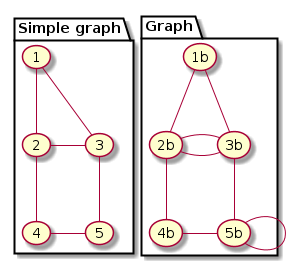
\includegraphics[scale=0.5]{ressources/images/GraphSimpleGraph.png}
            \caption{Simple graph $\Leftrightarrow$ Graph}
            \label{Simple graph & Graph}
        \end{figure}

\section{Type of graph}
    \subsection{Isomorphism}
        2 graphs G and H are isomorphic is $\exists \phi : V(G) \cup E(G) \rightarrow V(H) \cup E(H)$ bijective, such that:
        \begin{enumerate}
            \item $\phi(v)\in V(H)$ with $v\in V(G)$
            \item $\phi(e)\in E(H)$ with $e\in E(G)$
            \item $e\underset{G}{\sim}v \iff \phi(e)\underset{H}{\sim}\phi(v)$
        \end{enumerate}
    \subsection{Complete graph ($K_n$)}
        A complete graph is a simple graph with n vertex (for $K_n$) suc that every pair of distinct vertex are adjacent\\
        \begin{figure}[h]
            \centering
            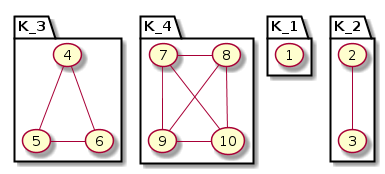
\includegraphics[scale=0.5]{ressources/images/CompleteGraphs.png}
            \caption{Every complete graph from $K_0$ to $K_4$}
            \label{Complete graph}
        \end{figure}
    \subsection{Subgraph}
        A graph H is a subgraph of G if:
        \begin{enumerate}
            \item $V(H)\subseteq V(G)$
            \item $E(H)\subseteq E(G)$
            \item  $\forall e \in E(H)$, the set of ends of $e$ in $H$ is equals to the set of ends in G
        \end{enumerate}
    \subsection{Spanning subgraph}
        A subgraph $H$ of $G$ is spanning if $V(H)=V(G)$
    \subsection{subgraph}
        A subgraph $H$ of $G$ is spanning if $V(H)=V(G)$

\section{Operations}
    \subsection{Deletetion}%TODO
    \subsection{Contraction}
        $G/e$ is the subgraph obtained from $G$ bydeleting $e$ and identitfying the 2 ends of $e$\\
        $|E(G)|=|E(G/e)|-1$\\
        $|V(G)|=|V(G/e)|-1$ (if e is not a loop)\\
        \begin{figure}[h]%TODO
            \centering
            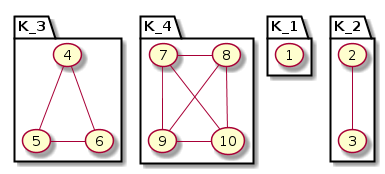
\includegraphics[scale=0.5]{ressources/images/CompleteGraphs.png}
            \caption{Every complete graph from $K_0$ to $K_4$}
            \label{Complete graph}
        \end{figure}
    \subsection{Minor}
        $H$ is a \textbf{minor} of $G$ if $H$ can be obtained from $G$ by deleting edges/vertices and contracting edges
    \subsection{Subdivision}
    $H$ is a \textbf{subdivision} of $G$ if $H$ can be obtain by subdivising somme edges of $G$\\
    $H$ is a \textbf{subdivision} of $G$ if $H$ can be obtained from $G$ by replacing each edge with a path of length $\geq 1$
        \begin{figure}[h]
            \centering
            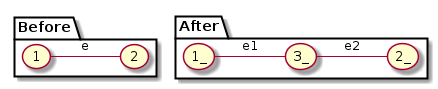
\includegraphics[scale=0.5]{ressources/images/SubDivision.png}
            \caption{Every complete graph from $K_0$ to $K_4$}
            \label{Complete graph}
        \end{figure}
    \subsection{Topological minor}
        $H$ is a \textbf{topological minor} of $G$ if a subdivision of $H$ is a subgraph of $G$\\
            \[\begin{array}{ccccc}
                \text{Subgraph} & \Rightarrow & \text{topological minor} & \Rightarrow & \text{minor}\\
                & \not\Leftarrow & & \not\Leftarrow & 
            \end{array}\]

